\section{Results and Discussion}
In this section we report the results obtained from the label-assignment step described in Section \ref{subsec:Label-Assignment} and the final model fit described in Section \ref{subsec:full_model}, using the covariates selected in
Chapter \ref{sec:variable_selection}. Moreover, Appendix C presents a validation study on synthetic data, illustrating the model’s performance.

\subsection{Posterior Cluster Allocation}
\label{subsec:clusters}

Following Section \ref{subsec:Label-Assignment}, we generated posterior draws of the latent allocation labels and summarized the clustering structure in a label-invariant way through the posterior similarity matrix (PSM) and a point estimate of the partition obtained via Binder loss.\\

The posterior evidence indicates that the model assigns all provinces to a single cluster. Equivalently, the estimated partition has $C=1$ non-empty component, so that no spatially distinct groups with different regression effects are detected. In practical terms, this means that the data do not support heterogeneous covariate effects across provinces under the proposed mixture/CAR specification and prior settings.\\

Given $C=1$, the full hierarchical model in Section \ref{subsec:full_model} reduces to a standard spatial regression with a single global coefficient vector $\beta$ (and residual scale $\sigma$), while spatial dependence is captured by the CAR random effect $\phi$:
\begin{align}
y_i^* \mid \alpha,\beta,\phi_i,\sigma &\sim \mathcal{N}\!\left(\alpha + x_i^{*\top}\beta + \phi_i,\ \sigma^2\right),
\qquad i=1,\dots,N.
\end{align}
All posterior summaries reported in the following sections refer to this $C=1$ fit.

\subsection{Posterior Inference}

\subsubsection{Predictors}

Table~\ref{tab:post_betas} reports posterior summaries for the intercept and regression coefficients associated with the covariates selected in Chapter \ref{sec:variable_selection}.

\begin{table}[!ht]
\centering
\begin{tabular}{lrrrrr}
\toprule
Parameter & Mean & SD & 5\% & 50\% & 95\% \\
\midrule
Intercept ($\alpha$) & 0.053 & 0.021 & 0.020 & 0.053 & 0.087 \\
private\_coverage & 0.104 & 0.037 & 0.044 & 0.105 & 0.165 \\
fem\_maj\_empl\_rate & -0.080 & 0.031 & -0.130 & -0.081 & -0.029 \\
public\_coverage & 0.151 & 0.034 & 0.095 & 0.150 & 0.206 \\
service\_empl\_rate & -0.059 & 0.031 & -0.110 & -0.059 & -0.008 \\
graduate\_mobility\_rate & 0.254 & 0.046 & 0.177 & 0.255 & 0.327 \\
empl\_growth & 0.051 & 0.027 & 0.007 & 0.051 & 0.094 \\
\bottomrule
\end{tabular}
\caption{Posterior summaries for intercept and regression coefficients.}
\label{tab:post_betas}
\end{table}

Figure~\ref{fig:dens_betas} shows posterior density estimates for the regression coefficients. This visualization complements Table~\ref{tab:post_betas}.\\

\begin{figure}[!ht]
\centering
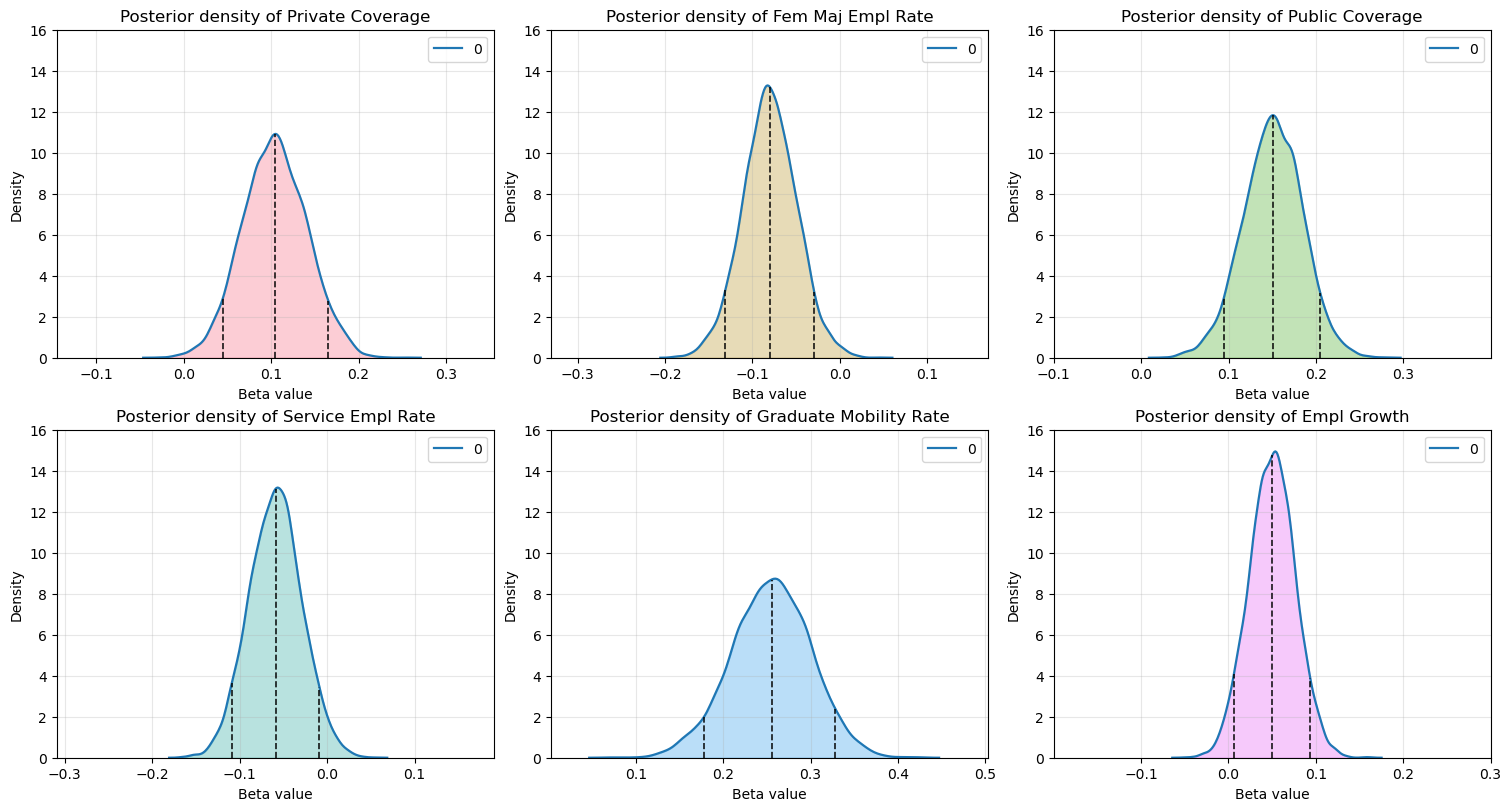
\includegraphics[width=\textwidth]{chapters/images/posterior-density-plots.png}
\caption{Posterior densities for the intercept and regression coefficients.}
\label{fig:dens_betas}
\end{figure}


According to Table~\ref{tab:post_betas} and Figure~\ref{fig:dens_betas}, the covariate showing the strongest positive association is the \texttt{graduate\_mobility\_rate}. This result is plausible, as female employment rates tend to be higher in provinces containing large urban areas with abundant job opportunities, which are also characterized by higher graduate mobility.\\

In addition, both private and public coverage variables are likewise positively correlated with the female employment rate. This finding was expected and it's encouraging for our study, although it does not allow us to establish a causal relationship between coverage and the increase in female employment.\\

In contrast, \texttt{fem\_maj\_empl\_rate} and \texttt{service\_empl\_rate} appear to be negatively correlated with female employment. However, compared with the other predictors, these effects are less significant.\\


\subsubsection{Spatial effect}

The response exhibits strong spatial autocorrelation. To interpret CAR random effect $\boldsymbol\phi$, we compare its posterior mean with the observed response.
Figure~\ref{fig:phi_vs_y} reports the posterior mean map of $\mathbb{E}[\phi_i\mid y]$, and the province-level \texttt{fem\_empl\_rate}. Provinces with positive (negative) $\phi_i$ correspond
to areas where the employment rate is systematically higher (lower) than what is explained by the selected covariates alone, after accounting for overall intercept and noise. In other words, $\boldsymbol\phi$ captures residual spatial patterns not explained by the included predictors.

\begin{figure}[!ht]
\centering
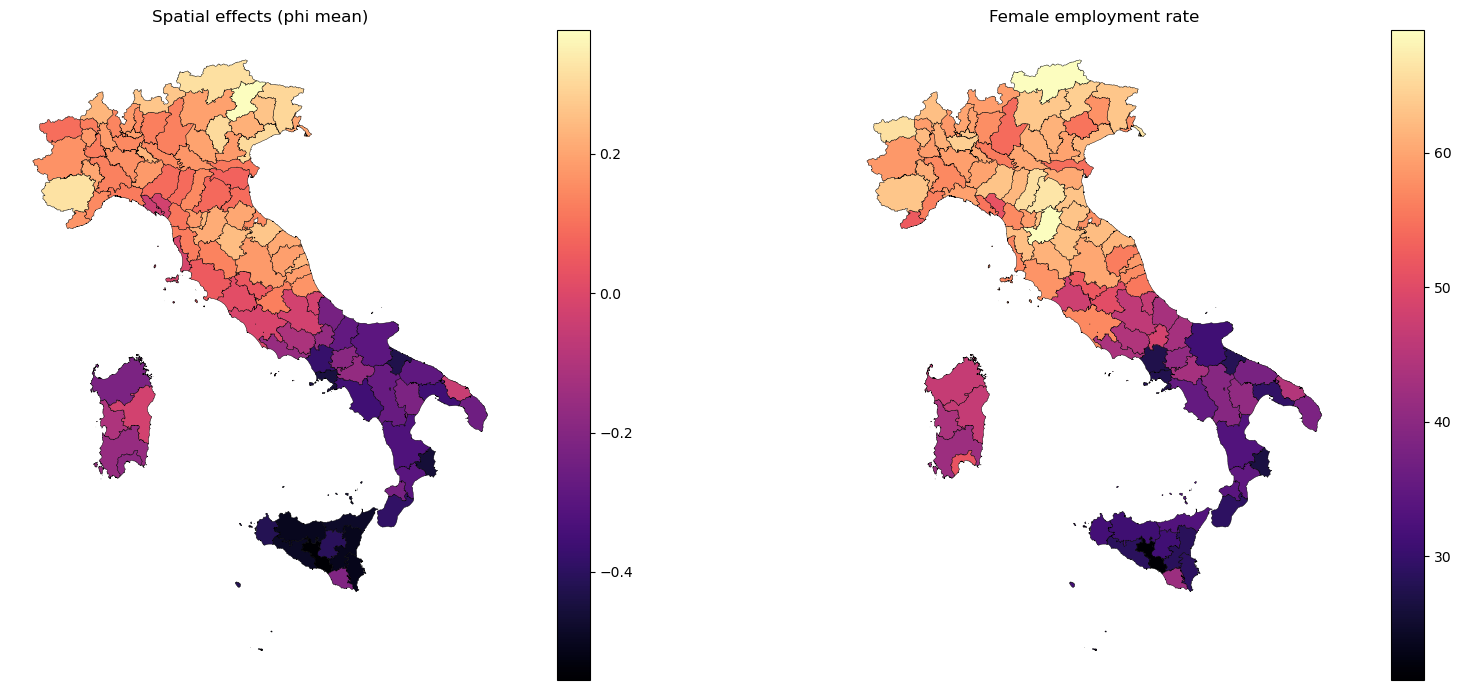
\includegraphics[width=0.85\textwidth]{chapters/images/car-vs-fem.png}
\caption{Posterior mean of the spatial random effects $\boldsymbol\phi$ (left) and Observed female employment rate by province (right).}
\label{fig:phi_vs_y}
\end{figure}

From Figure~\ref{fig:phi_vs_y}, we observe that the spatial effect across Italy follows the same overall trend as the female employment rate, with a gradual divide between the northern and southern provinces. This suggests the presence of a significant underlying structure that is not explained by the selected predictors. 